\documentclass{standalone}
\usepackage{pgfplots}
\pgfplotsset{compat=1.18}

\begin{document}

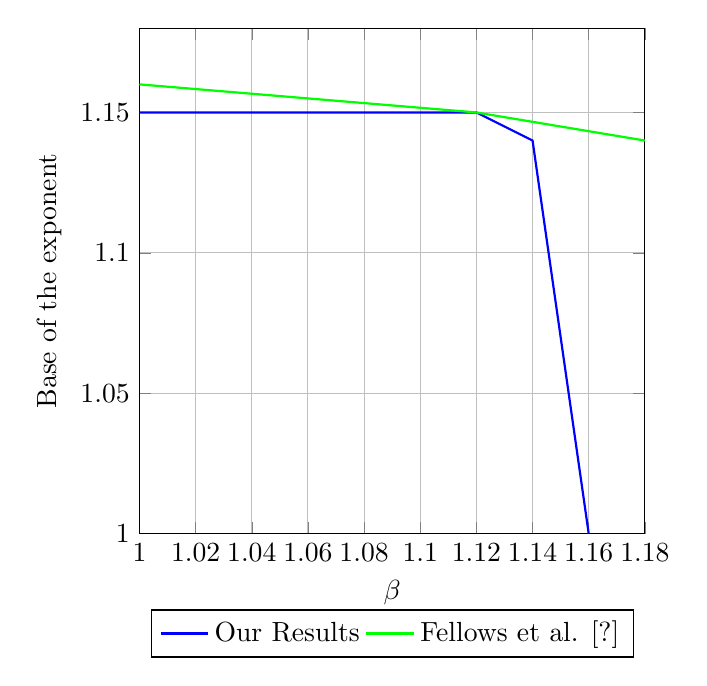
\begin{tikzpicture}
\begin{axis}[
    width=8cm,
    height=8cm,
    grid=both,
    xlabel={$\beta$},
    ylabel={Base of the exponent},
    ymin=1,
    ymax=1.18,
    xmin=1,
    xmax=1.18,
    xtick={1, 1.02, 1.04, 1.06, 1.08, 1.1, 1.12, 1.14, 1.16, 1.18},
    ytick={1, 1.05, 1.1, 1.15},
    legend style={at={(0.5,-0.15)},anchor=north,legend columns=-1},
    legend cell align={left},
]

\addplot[
    blue,
    thick,
] coordinates {
    (1.0, 1.15)
    (1.12, 1.15)
    (1.14, 1.14)
    (1.16, 1.0)
};

\addplot[
    green,
    thick,
] coordinates {
    (1.0, 1.16)
    (1.12, 1.15)
    (1.18, 1.14)
};

\legend{Our Results, Fellows et al. [?]}
\end{axis}
\end{tikzpicture}

\end{document}